
%(BEGIN_QUESTION)
% Copyright 2015, Tony R. Kuphaldt, released under the Creative Commons Attribution License (v 1.0)
% This means you may do almost anything with this work of mine, so long as you give me proper credit

The following is an electrical schematic diagram for a three-phase 50/51 overcurrent protective relay circuit, where three overcurrent relays (one for each phase of the power circuit) trip a single breaker in the event of an overcurrent fault.  The power diagram on the left shows all the high-voltage components, while the control diagram on the right shows the circuitry associated with the breaker's trip coil:

$$\includegraphics[width=15.5cm]{i01971x01.eps}$$

Examine this schematic diagram, and then explain how the circuit breaker may be tripped by {\it any one} of the three overcurrent relays.  Also, identify at least one circuit fault in either the power diagram or the control diagram that could prevent the circuit breaker from tripping when it needs to.

\vskip 10pt

Finally, calculate the amount of voltage dropped by the instantaneous sensing coil of one of the relays (coil 50-1, coil 50-2, or coil 50-3) when line current is 1300 amps at 60 Hz, assuming a 2000:5 CT ratio for each line, and given a coil resistance of 31.35 milliohms and a coil inductance of 27.33 microhenrys:

\vskip 10pt

$V_{coil}$ = \underbar{\hskip 50pt} volts




\vskip 20pt \vbox{\hrule \hbox{\strut \vrule{} {\bf Suggestions for Socratic discussion} \vrule} \hrule}

\begin{itemize}
\item{} Explain the purpose of the circuit breaker's {\it 52a} contact shown in the control diagram.
\end{itemize}

\underbar{file i01971}
%(END_QUESTION)





%(BEGIN_ANSWER)


%(END_ANSWER)





%(BEGIN_NOTES)

Each protective relay monitors current through one of the power lines.  The trip contacts of each relay are paralleled with one another, so that only one of them needs to trip in order to send 125 VDC station power to the circuit breaker's trip coil.

\vskip 10pt

Any {\it open} fault in the control diagram circuit that's in series with the breaker trip coil would prevent the breaker from tripping when needed.

\vskip 30pt

When line current is 1300 amps, each CT will reduce that current to a much smaller value through the relay's sensing coils:

$$I_{CT} = \left({1300 \hbox{ A} \over 1} \right) \left({5 \over 2000} \right) = 3.250 \hbox{ A}$$

To calculate voltage drop across the instantaneous coil while carrying this current, we must first calculate the impedance of that coil from the given resistance and inductance values.  We know that $Z = \sqrt{R^2 + X_L^2}$ for a series resistor-inductor network, so:

$$X_L = 2 \pi f L = 2 \pi (60)(27.33 \times 10^{-6}) = 10.3 \hbox{ m} \Omega$$

$$Z = \sqrt{R^2 + X_L^2} = \sqrt{\left(31.35 \times 10^{-3}\right)^2 + \left(10.3 \times 10^{-3} \right)^2} = 33.3 \hbox{ m} \Omega$$

Now, we may apply Ohm's Law to calculate voltage dropped across the coil:

$$V = IZ = (33.3 \hbox{ m} \Omega) (3.250 \hbox{ A}) = 107.25 \hbox{ mV}$$











\vfil \eject

$$\includegraphics[width=15.5cm]{i01971x02.eps}$$

\vskip 20pt \vbox{\hrule \hbox{\strut \vrule{} {\bf Virtual Troubleshooting} \vrule} \hrule}

This question is a good candidate for a ``Virtual Troubleshooting'' exercise.  Presenting the diagram to students, you first imagine in your own mind a particular fault in the system.  Then, you present one or more symptoms of that fault (something noticeable by an operator or other user of the system).  Students then propose various diagnostic tests to perform on this system to identify the nature and location of the fault, as though they were technicians trying to troubleshoot the problem.  Your job is to tell them what the result(s) would be for each of the proposed diagnostic tests, documenting those results where all the students can see.

During and after the exercise, it is good to ask students follow-up questions such as:

\begin{itemize}
\item{} What does the result of the last diagnostic test tell you about the fault?
\item{} Suppose the results of the last diagnostic test were different.  What then would that result tell you about the fault?
\item{} Is the last diagnostic test the best one we could do?
\item{} What would be the ideal order of tests, to diagnose the problem in as few steps as possible?
\end{itemize}








\filbreak

\vskip 20pt \vbox{\hrule \hbox{\strut \vrule{} {\bf Virtual Trip-testing} \vrule} \hrule}

This question is a good candidate for a ``Virtual Trip-testing'' exercise.  Presenting the diagram to students, you pose an assignment whereby students must figure out how to test some component of this system to check that it will operate as intended to shut down the system in an abnormal (trip) condition, with some realistic limitation (e.g. power cannot be shut off to the load).  Students then propose various methods for executing the test.  Your job is to determine whether or not their proposed tests will achieve the desired result(s).

During and after the exercise, it is good to ask students follow-up questions such as:

\begin{itemize}
\item{} Where might our planned test strategy go wrong?  In other words, what thing(s) might happen to foil our test, either to invalidate the results or to not honor the stated limitation(s)?
\item{} Suppose the limitation were different.  How would this affect our ability to carry out the test?
\item{} Is the last test strategy best one we could execute?
\end{itemize}


%INDEX% Electric power systems: protective relays (time-overcurrent)
%INDEX% Protective relay: instantaneous overcurrent (50)
%INDEX% Protective relay: time-overcurrent (51)
%INDEX% Safety, shutdown system: trip testing (protective relay circuit)

%(END_NOTES)


